\chapter{Conclusions and Future Directions}
\label{chap:chapter5}
\section{Chapter \ref{chap:chapter2} - Multi-state design and polyspecificity}
I expand on the limitations of \rosettadesign~by looking at the imperfect agreement between what we expect \rosettadesign~to recovery and what was actually observed. I bin these into three categories, mature sequence bias, evolutionary sequence bias, and incomplete ensemble bias. Section \ref{sec:maturebias} accounts for mature sequence bias, which may be the most abstract concept. When a residue is ``important'' for most of the antibody-antigen complexes, it should be recovered often. However if it only is important in a few complexes, then any given residue can meet the design challenges for the complexes in which it is not important.

Section \ref{sec:evobias} refers to evolutionary sequence bias. Here we may see imperfect agreement with the design and actual antibody sequence simply because the antibody has not achieved maximal potency. \rosettadesign~may have selected better amino acid sequences for the epitope. Given enough time to for complete antibody evolution, the sequence may have matched. This is founded on the principle that \rosettadesign~gives the best sequence for any design challenge.

Section \ref{sec:limits} gives the limits of computation including the finite ensemble size that states there are not enough PDBs to compensate for ``structural space'' that \rosettadesign~samples. This section also details some of the more classic limitations including the limits of the \rosetta~scoring function and limitations of the sampling algorithms. In the future this may be ameliorated with more structures being deposited to the PDB, and improvements to the scoring function including explicit solvent modeling.

The power of chapter \ref{chap:chapter2} is in the future directions. While we use multi-state design to interrogate the flexibility of the germline repertoire, the end goal was always to design cross-binding antibodies. Many pathogens which evade traditional vaccination do so by evolving multiple serotypes or antigenic variants that encompass a tremendous sequence space. HIV, Influenza and dengue virus (DENV) are such examples of antibodies that use antigenic variation as a means to evade a broadly protective immunogenic response. It is to these pathogens that a broad cross-reactive response will be critical \citep{Corti:2013ex,Lanzavecchia:2009dd,Corti:2011ku,Simonelli:2013jc}. Multi-state design will be invaluable in the design of these antibodies. Consider \ref{fig:fig5_1}, here we take a known cross-reactive group 1 antibody against influenza known as CR6261 \citep{Throsby:2008dc} which does not bind to Influenza type B.

\begin{figure}[!t]
   \centering
   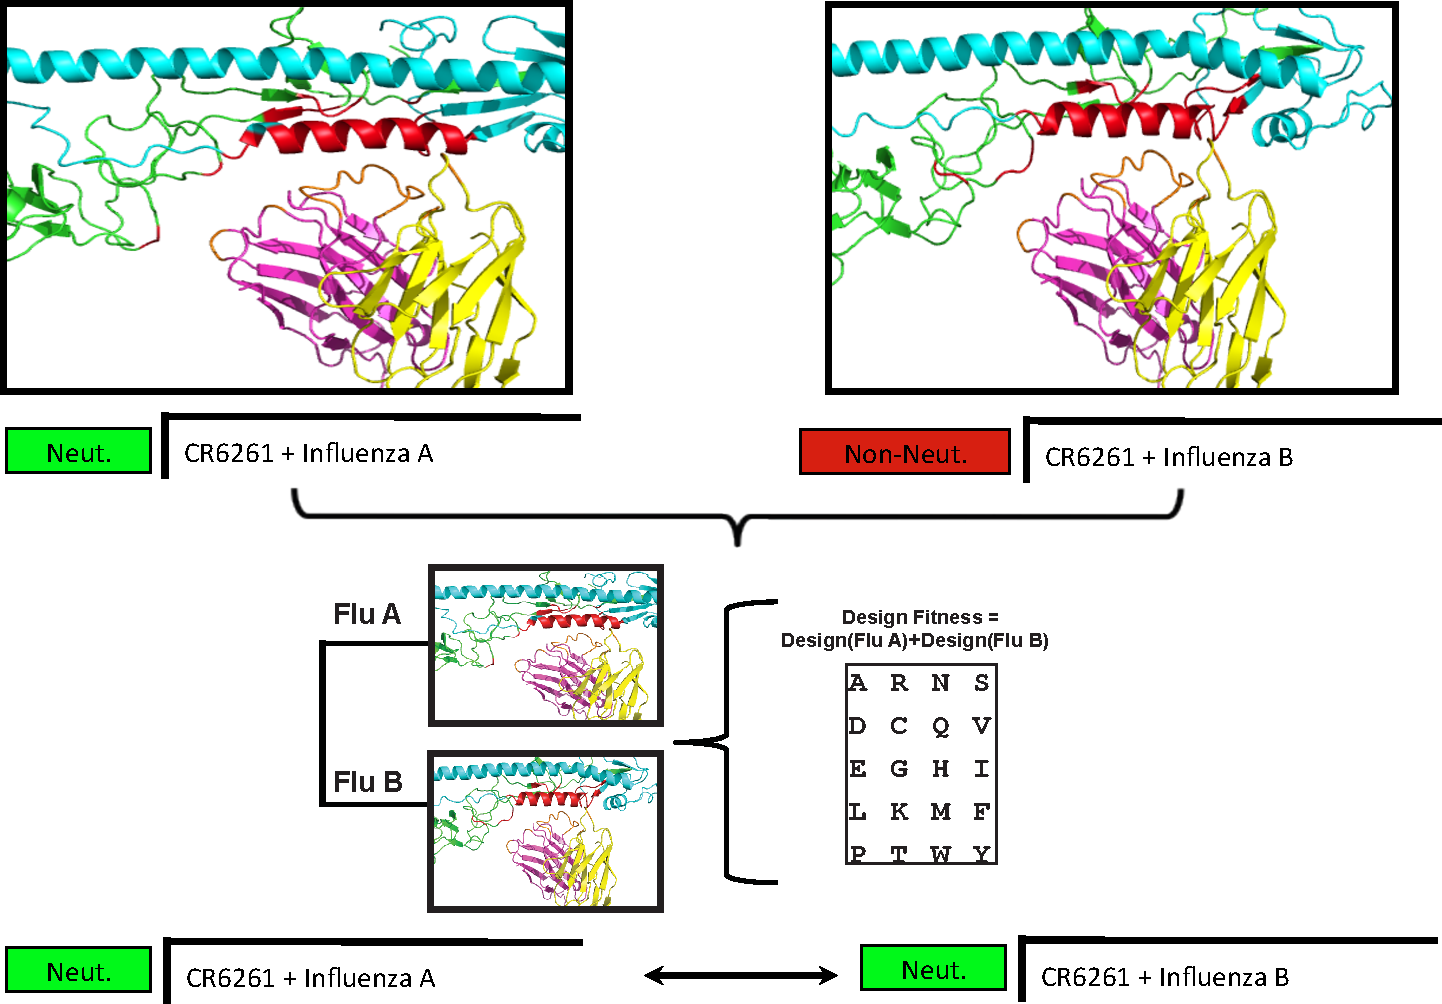
\includegraphics[width=\columnwidth]{images/chapter5/figure5_1.pdf}
   \caption[Multi-State Design of Broadly Neutralizing Influenza Antibodies]{Multi-state design of broadly neutralizing influenza antibodies. Initially, the antibody CR6261 only binds and neutralizes only Influenza A subtypes. Using multi-state design I plan to make minimal mutations at the interface that allow binding to Influenza type B while retaining binding to Influenza type A. This principle allows me to design in cross-specificity.}
       \label{fig:fig5_1}
\end{figure}


I even took this idea into the lab looking at special cases for influenza antibody. I considered the antibody CR6261 as it was bound to the stem portion of influenza \citep{Corti:2011ku}. At the stem region, their is less conformational diversity. I hypothesized that this epitope loses neutralization affinity due to point mutations at the interface rather than large conformational shifts that are evident in the head region. This would be easier for \rosettadesign~to recover. First, I wanted to create a proof-of-concept by seeing if we can enhance specificity to already known binders. I chose H1/South Carolina/1918 and H5/Vietnam/2004 pandemic strains as both had a crystal structure bound to CR6261. Using multi-state design, I told \rosettadesign~to enhance binding to both variants. Figure \ref{fig:fig5_2} shows the design process. The sequence logo in (A) shows the amino acids preferred at the interface. For (B), we analyzed the fitness of each mutation as either having beneficial or deleterious effects. If it enhanced fitness for both H1 and H5, we made the mutations in the laboratory. They indeed did enhance binding to both variants compared to wild-type CR6261 (figure \ref{fig:fig5_2} C.).

\begin{figure}[!t]
   \centering
   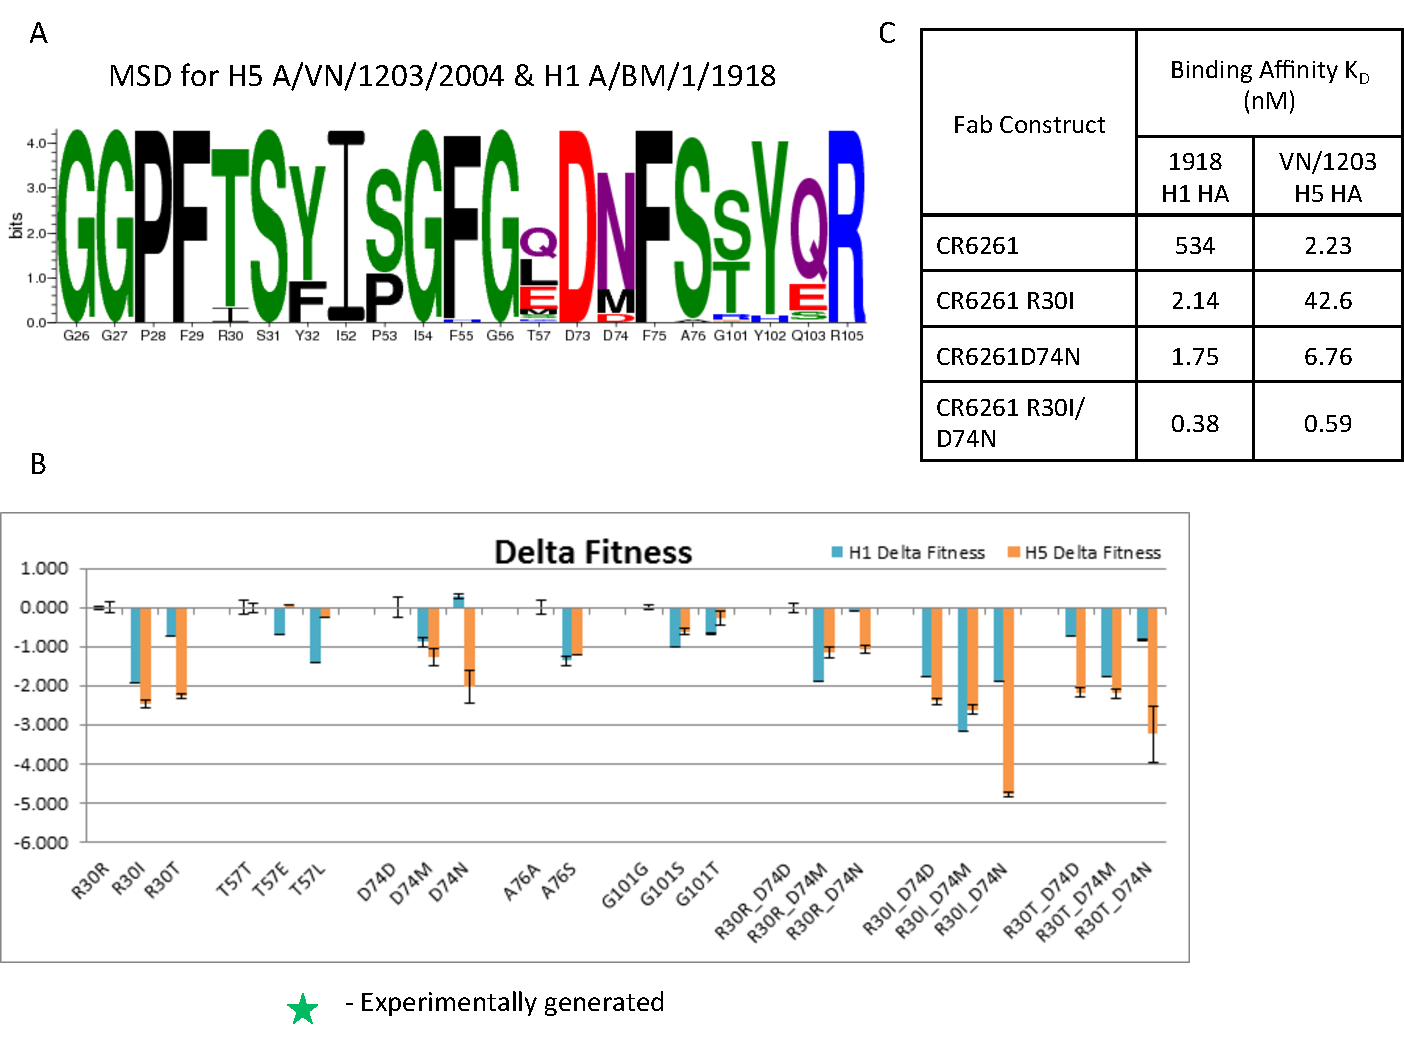
\includegraphics[width=.9\textwidth]{images/chapter5/figure5_2.pdf}
   \caption[Preliminary for MSD Proof-of-Concept]{Preliminary for MSD proof-of-concept. A sequence logo for all positions considered for redesign at the interface. Higher letters indicate \rosetta's proclivity for a certain amino acid sequence (A). Fitness analysis of each position is a sum of stability and binding energy. Lower energies indicate better fitness. Ideally, both H1 and H5 would have decreased fitness energy. Stars indicate mutations that were made experimentally (B). The binding affinities from the suggested mutations from \rosetta. The double mutant gives the best binding affinity (C).}
       \label{fig:fig5_2}
\end{figure}

Of course this proof-of-concept can extend well beyond influenza. My plan was to use this to get a serotype specific antibody to bind (and therefore, potentially neutralize) cross-serotype, cross-group, and cross influenza sub-type. However, many labs are trying to design cross-reactive antibodies. One advantage of multi-state design is that if you fine-tune specificity you do not have to lose specificity to your original epitope. For example, in a paper by Simonelli \textit{et al.} \citep{Simonelli:2013jc}, they used computational modeling along with NMR restraints to place give a molecular definition of an anti-DENV against all four DENV serotypes. They then used their knowledge of rationale design to fine tune specificity to each serotype individually. However, upon making one mutation specific to a given serotype often abrogated binding to the others. Therefore it is possible to enhance breadth at the cost of specificity. This type of problem is ideal for multi-state design as it can fine tune specificity without predicted loss of binding to your original epitope.

In related work, structural viral homologs could also be used in multi-state design. For example, an antibody found in chronically exposed repository infected patients bound and neutralized four different paramyxoviruses, human respiratory syncytial virus (HRSV), human metapneumovirus (HMPV), bovine RSV (BRSV) and pneumonia virus of mice (PVM) \citep{Corti:2013cv}. This antibody was found by screening a common structural homolog (prefusion protein F) against anti-HRSV screened from over 200 donors to narrow down their search. I hypothesize that this type of structural information can be used in multi-state design to make \textit{de novo} designed cross-neutralizers much the way nature selected cross-neutralizers from these patients.

Finally, there is much use for this algorithm's fitness function. While I describe antibody design in the context of \textit{designing for} a certain antigen, it may be beneficial to \textit{design against}. I can modify the scoring function in such a way where we select mutations that will \textit{design for} one antigen, and \textit{design against} others. This allows any fine tuning of specificity changes that are needed against antibodies while not compromising the structural integrity of the immunoglobulin fold. I can imagine this will be an invaluable tool for designing against antigens that are found to be related to autoimmunity.

\section{Chapter \ref{chap:chapter3} - Broadly neutralizing antibodies from HIV-\naive~donor repertoires}
In chapter \ref{chap:chapter3}, I used antibody design to interrogate the HIV-\naive~repertoire to answer a simple question for the paradigms of HIV vaccinology. How close is the \naive~donor repertoire to eliciting neutralizing antibodies? I used the principles guided by both reverse  and forward vaccinology \citep{Burton:2012bh}. Reverse vaccinology principles require that the broadly neutralizing antibodies are first characterized from chronically infected patients. I used the the V1/V2 binding antibody PG9 that was discovered in a chronically infected African donor \citep{McLellan:2011dg,Walker:2009cd}. This is where I introduced a new paradigm into vaccinology. Rather than used structure based immunogen design from the PG9 epitope which has been characterized, I instead investigated the healthy donor repertoire. In my early work here, I had helped discover long HCDR3s in healthy donors, and it was with this information I wanted to pursue this question.

I conclude that although there are some antibodies from the HIV-\naive~donor repertoire that are able to mimic PG9 hammerhead like configuration, there are very few from our population pool. Even those that we did find needed some amounts of mutation that honed specificity to make these antibodies truely binding and neutralizing.

There is an absolute limitation to this study, and that is the amount of long-HCDR3 sequences we started with. Out of one-half-billion sequences, we only were able to obtain ~26,000 unique 30-length sequences that were viable in our study. That is an incredibly low amount. Along with Andy Fire, Jessica Finn and myself, we have devised new clever experiments that can potentially enrich for long HCDR3s. We have noticed that in this study and previous studies, that most antibodies with long HCDR3s contain a J\textsubscript{H}6 gene segment \citep{Briney:2012ib}. In addition, PG-type antibodies often use V\textsubscript{H}3-30 genes. This makes the initial PCR rounds for gene-specific targeting a simple task. Rather than use ambiguous primer-sets for all gene families, I plan to use just specific primers to J\textsubscript{H}6 and V\textsubscript{H}3-30 for amplification of B-cell mRNA transcripts. I can actually predict that this will enhance the mean HCDR3 length from 15.56 to 18.06 (figure \ref{fig:fig5_3}). In addition, new advances in high resolution gel electrophoresis allow single base pair resolution and purification. That would allow only very-long HCDR3 sequences to be purified and enriched from the canonical length background. Using this, I could truly use this population pool in my newly created bioinformatics pipeline to test the HIV-\naive donor sequences.

\begin{figure}[!t]
   \centering
   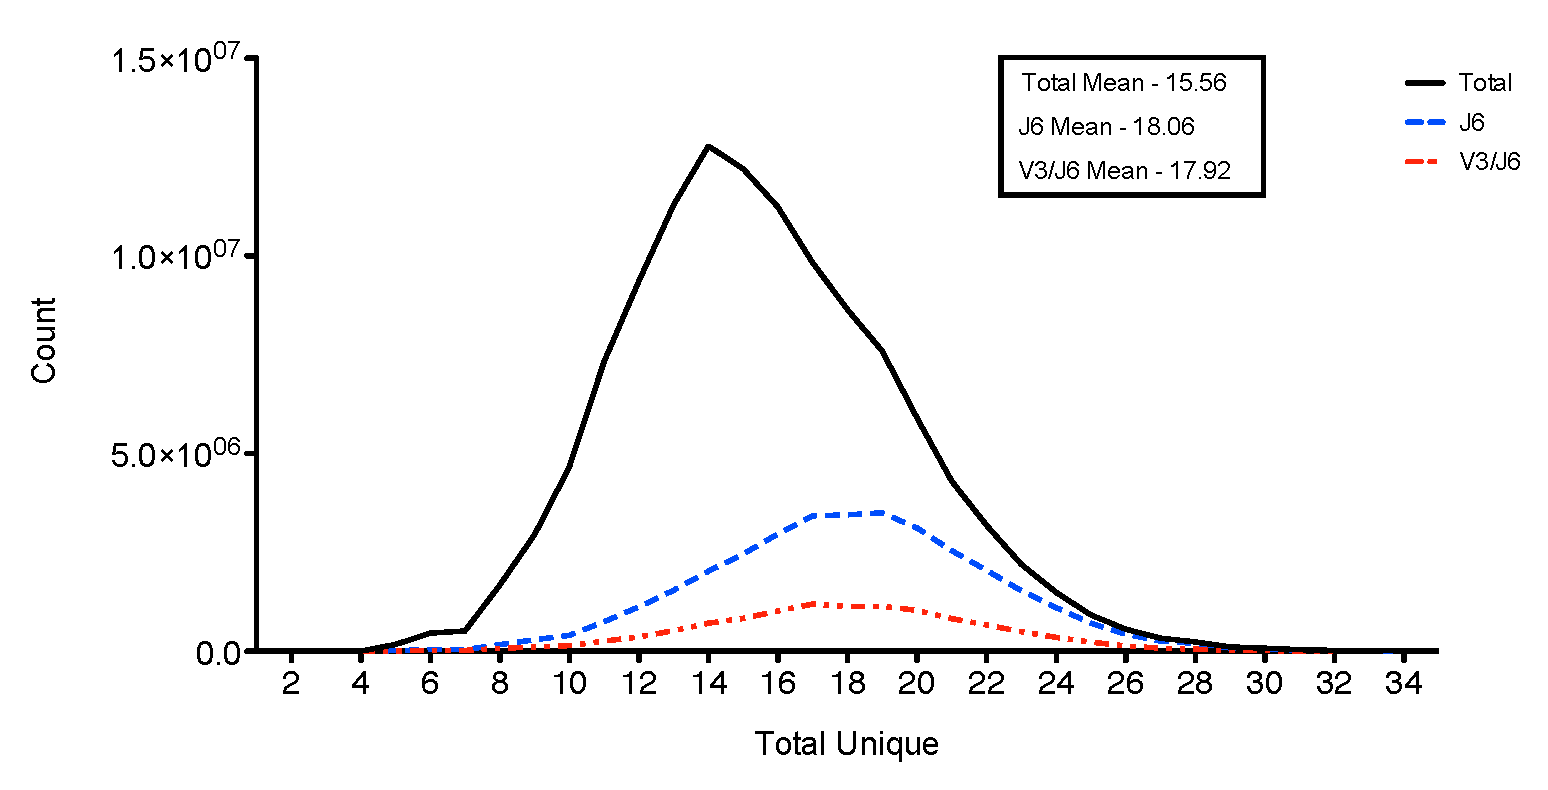
\includegraphics[width=.9\textwidth]{images/chapter5/figure5_3.pdf}
   \caption[HCDR3 of J\textsubscript{H}6 Gene Families]{HCDR3 of J\textsubscript{H}6 gene families. A distribution curve for HCDR3 sequences is shown for all VDJ familes (black). When only J\textsubscript{H}6 genes are considered, the mean length shifts from 15.56 to 18.06. If only J\textsubscript{H}6 and V\textsubscript{H}3 gene families are considered the mean shifts down to 17.92.}
       \label{fig:fig5_3}
\end{figure}

One problem that is mentioned is the potential framework bias. Although it has been demonstrated that the HCDR3 loop is responsible for a majority of the contact and by extension the mechanism of neutralization \citep{Pejchal:2010fp,Pancera:2010hh}, it can't be ruled out that the framework provides some contribution to binding in the LHCDR3 and HCDR2 region \citep{McLellan:2011dg}. However, in recent studies, mutations all the way back to germline have shown that these mutations aren't absolutely necessary necessary to necessitate binding and by extension neutralization \citep{Klein:2013iz}. In chapter \ref{chap:chapter2}, we find at least fifty percent of the the germline framework may be necessary for binding, even those residues that lie extremely distal to the interface. This leads me to believe in an inherent framework bias in our study. I used PG9 framework as the complete sequence to the rest of the heavy chain and the light chain was unknown (the current technology is limited at the time of writing). But other studies show us that surrounding mutations of the HCDR3 loop allow it to form its native conformation \citep{Wong:2011ff}. I want to know the effects of other germline frameworks on HIV-\naive~HCDR3 loops.

I proposed a display technology solution to this problem. If I can isolate 30-length (or longer) HCDR3 sequences from the B cell repertoire, I can engineer cloning sites into them as I have done for the PG9 framework. However, each cloning site will be slightly upstream of the HCDR3 site. In this manner we can use any germline framework to test each HIV-\naive~conformation. In this way, we can test inherit framework bias from each germline framework on the healthy HCDR3 sequence. For the amount of HCDR3 sequences I get (roughly estimate 100,000 using the technique described above), I can test this on each V\textsubscript{H} gene family, giving 5.2 million different combinations of antibodies I can test and remove framework bias. In addition, I can combine germline light chain repertoires to increase our combinations. I feel like this would be like an incredibly useful experiment to find antibodies from HIV-\naive~donors with the absolute minimum amount of mutations. In this way I can get an absolute threshold to describe what a vaccine will need to elicit using a very inexpensive technology.

\section{Chapter \ref{chap:chapter4} - Broadly neutralizing antibody redesign}
I indicate some of the issues with redesign and highlighted them in the publication that accompanies chapter \ref{chap:chapter4}. For instance, \rosettadesign, indicated that D115N would be the most beneficial mutation. When I characterized this mutation experimentally, I found this mutation to actually hinder binding. This is due to some of the limitations of \rosetta~that have been discussed at length, especially in chapter \ref{chap:chapter2} where I discuss the limits of the \rosetta~scoring function. This is being addressed by a large number of \rosetta~collaborators in the Commons with more accurate representation of hydrogen bondings and explicit solvent models.

The excitement of future endeavors with the redesign of antibodies is the most exciting and probably one of the most straight forward future directions I have. For one, this type of design which we applied to PG9 can be applied to any antibody, whether it be broadly neutralizing or modestly potent. \rosetta~allows us to tailor the scoring function to \textit{design for} stability or binding energy, which we have found to be a necessary component to increasing potency and breadth of contemporary antibodies.

One step I have taken with future directions, is applying the same methodology to PG9s sister antibody PG16. In figure \ref{fig:fig5_4}, an initial pilot study using the same redesign methodology has been performed. As is evident, some of the PG16 variants are able to bind BaL gp120 monomers with greater affinity. There is a huge caveat at the current time of this study. These PG16 HCDR3 loops were put on the PG9 backbone with the exception of PG16\textit{wt}. The PG9 framework may be responsible for the antibody binding BaL gp120 monomer. I have begun taking these constructs and putting them on PG16 backgrounds to see if there is difference in PG9/PG16 backbone. If there is, that gives plausibility to framework bias as discussed above.

\begin{figure}[!t]
   \centering
   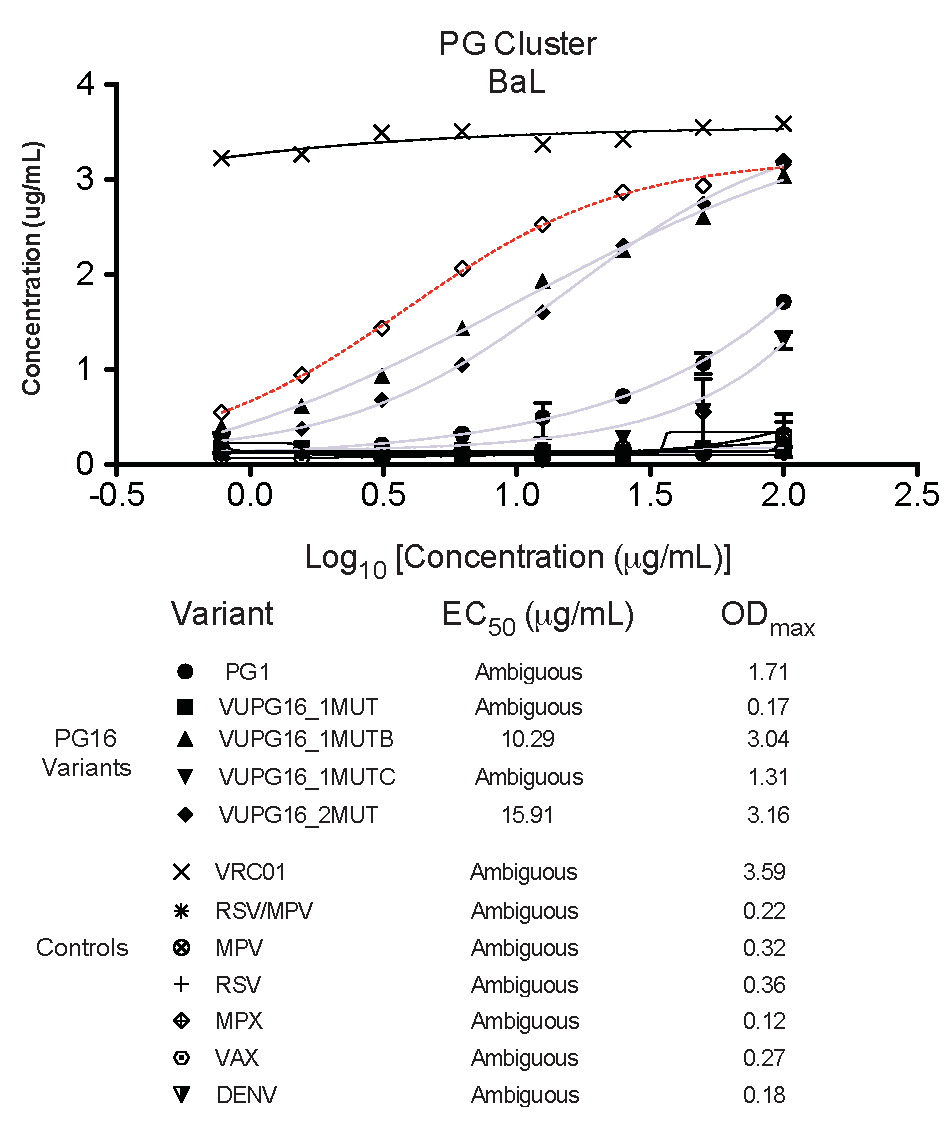
\includegraphics[scale=.5]{images/chapter5/figure5_4.pdf}
   \caption[Binding Profile of PG16 Variants]{An initial pilot study with PG16 HCDR3 variants on a PG9 backbone. All the variants have a PG9 backbone except for PG16\textit{wt} which may explain the strength in binding. Various negative and positive controls are shown for other viral species.}
    \label{fig:fig5_4}
\end{figure}

The future for antibody redesign is staggering, especially in context of evolutionary sequence bias as introduced above. Researchers isolate antibodies in the middle of their evolutionary cycle where they may not be optimized for potency and breadth, only the ability to bind and not necessarily to a threshold. With the redesign principles that we have gained insight into with PG9 redesign, it opens up an exciting new avenues for any antibodies, and aids in understanding the principles that need to be considered for the grand challenge in antibody design, the \textit{de novo} design of a nM binder.

\section{Other Applications of Antibody Design}
My very first specific aim was to establish a correlation between \silico~binding energy and experimental binding energy. This was the start of a very tedious process of making diverse HIV antigen to test two broadly neutralizing antibodies VRC01, and b12 \citep{Wu:2009ks,Li:2011ea}. As I began reading the literature, most notably a study done by Kwon and colleagues \citep{Kwon:2012eo}, I noticed that the VRC01 bound gp120 was different from the b12 bound structure where the b12 bound structure is in the pre-CD4 bound state and VRC01 is in the CD4-bound state. I hypothesized that, VRC01 would be entropically limited because it would always need to change the conformation of gp120 in order to bind. However when it does so, it exposes an extremely conserved epitope.

To first test this hypothesis, I wanted a baseline of gp120 binding using ELISAs and \ec as a metric. Figure \ref{fig:fig5_5} panel A and B show these curves for many variants of gp120 for b12 and VRC01, respectively. I then started to use ITC to get a better metrics of how each antibody was binding (figure \ref{fig:fig5_5} C), and I found that VRC01 made many hydrogen bonding contacts, but gave up huge entropic penalties. Much work is needed on this front as an accurate ITC for each variant is absolutely necessary to confirm this hypothesis, but the initial work of creating constructs and protein has been done. It is also important to note that the reported literature values may be different from mine which again underlines the importance of in house experiments.

\begin{figure}[!t]
   \centering
   \includegraphics[width=\columnwidth]{images/chapter5/figure5_5.pdf}
   \caption[CD4 Binding mAbs Mechanisms of Escape]{CD4 binding mAbs mechanisms of escape. Binding ELISAS against clade B and C gp120 monomers for CD4 binding antibody b12 (A) and VRC01 (B). Isothermal titration calorimetry of VRC01 antibody against b12 highlighting enthalpic domination (C). Experimental vs. literature binding values show a weak correlation (D). Computational predicted binding energy for homology modeling of VRC01 and gp120 variants and b12 and gp120 variants correlates well for only b12.}
    \label{fig:fig5_5}
\end{figure}

With the \ec values, I can plot an \silico~binding energy vs. the experimental binding energy (figure \ref{fig:fig5_5}) and find that there is no correlation for VRC01 but good correlation for b12. This result is intriguing as the conformational shift is not accounted for in \rosetta~and there are probably many other states that gp120 samples. A mechanism of resistance has been worked out with brute force \citep{Li:2011ea}, but I would like to confirm \silico.

These results are very preliminary and would best be guided by ITC experiments for the rest of the variants, but much of the work has been done.

